\documentclass{cmn}

\def\scopeXSep{17.5mm}

\tikzset{
  tree/.style={
    level distance=8mm,
    level 1/.style={sibling distance=10mm},
    level 2/.style={sibling distance=8mm},
    every node/.style={draw,circle,inner sep=1.75mm}
  }
}

\begin{document}
  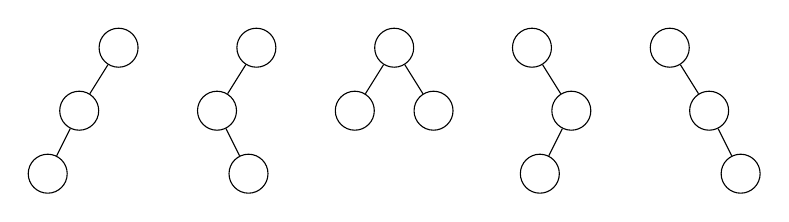
\begin{tikzpicture}
    \begin{scope}[tree]
      \node {}
        child {node {}
          child {node {}}
          child[missing]
        }
        child[missing];
    \end{scope}

    \begin{scope}[tree,xshift=\scopeXSep]
      \node {}
        child {node {}
          child[missing]
          child {node {}}
        }
        child[missing];
    \end{scope}

    \begin{scope}[tree,xshift=2*\scopeXSep]
      \node {}
        child {node {}}
        child {node {}};
    \end{scope}

    \begin{scope}[tree,xshift=3*\scopeXSep]
      \node {}
        child[missing]
        child {node {}
          child {node {}}
          child[missing]
        };
    \end{scope}

    \begin{scope}[tree,xshift=4*\scopeXSep]
      \node {}
        child[missing]
        child {node {}
          child[missing]
          child {node {}}
        };
    \end{scope}
  \end{tikzpicture}
\end{document}
